\newpage
\subsection{Fläche zwischen Funktionen}

Es soll die Fläche zwischen den beiden Funktionen ermittelt werden:
\begin{itemize}
    \item $\textcolor{blue}{f(x) = x^2+2}$
    \item $\textcolor{red}{g(x) = -x^2+5}$
\end{itemize} 

\hfill \break
Schritte:
\begin{enumerate}
    \item Schnittpunkte Berechnen: \begin{itemize}
        \item Ermittlung durch Gleichsetzen: $f(x) = g(x)$
        \item Ermittlung mit TR $2_{nd}$ calc intersect
    \end{itemize}
    \item Zwischen den ermittelten Schnittpunkten Integrieren: $\int\limits_{x2}^{x1} g(x)-f(x)dx$
\end{enumerate}

\hfill \break
Dabei sit zu beachten das immer die obere minus der unterren Kurve gerechnet werden muss.

\hfill \break
Example:\\
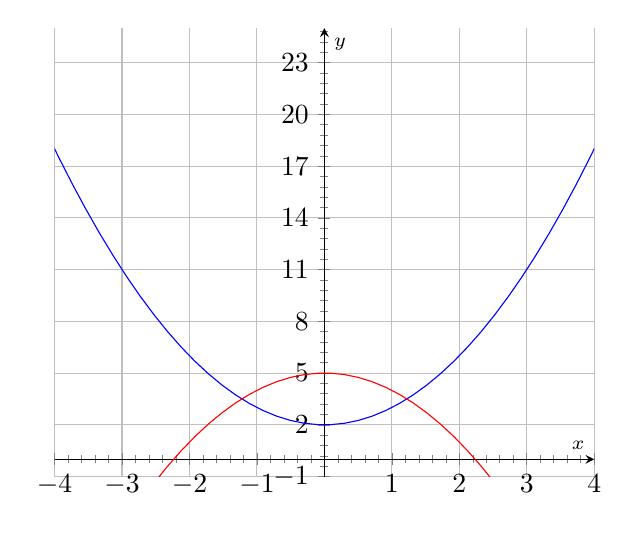
\begin{tikzpicture}[scale=1]
    \begin{axis}%
        [
            grid=major,
            xtick={-5,-4,...,4},
            minor x tick num=4,
            xmin=-4,
            xmax=4,
            xlabel={\scriptsize $x$},
            axis x line=middle,
            ytick={-1,2,...,25},
            minor y tick num=4,
            ymin=-1,
            ymax=25,
            ylabel={\scriptsize $y$},
            axis y line=middle,
            no markers,
            samples=100,
            domain=-10:10,
        ]
        \addplot[blue] (x,{x^2+2});
        \addplot[red] (x,{-x^2+5});
    \end{axis}
\end{tikzpicture}